\documentclass[conference,a4paper]{IEEEtran}
\pdfminorversion=6
\usepackage[T1]{fontenc}
\usepackage[utf8]{inputenc}
\usepackage{graphicx,booktabs,tabularx,amsmath,amssymb,tikz,cite}
\usepackage[table]{xcolor}
\usepackage{pgfplots}
\pgfplotsset{compat=1.18}
\usepgfplotslibrary{groupplots}
\usepackage[hidelinks]{hyperref}
\newcolumntype{Y}{>{\raggedright\arraybackslash}X}
\newcommand{\ind}{\mathbf{1}}
\begin{document}
\title{XBone-Net: Parameter-Efficient Radiograph Classification with Clinical History}
\author{\IEEEauthorblockN{%
Van-Le-Ba-Thanh Nguyen\textsuperscript{1,2},
Gia-Kiet Nguyen\textsuperscript{1,2},
Quoc-Ngoc Ly\textsuperscript{1,2},
Thi-Thanh-Ha Do\textsuperscript{1,2}}
\IEEEauthorblockA{%
\textsuperscript{1}Faculty of Information Technology, University of Science, Vietnam\\
\textsuperscript{2}Vietnam National University, Ho Chi Minh City, Vietnam\\
\{nvlbthanh22, ngkiet22\}@clc.fitus.edu.vn\\
\{lqngoc, dttha\}@fit.hcmus.edu.vn}}
\maketitle

\begin{abstract}
Clinical history complements skeletal radiographs, but adapting biomedical vision--language models to small, imbalanced cohorts requires effective fusion under limited training resources. Existing image--text pretraining provides transferable representations, while the downstream trade-off between classification performance and adaptation cost remains task dependent. We present XBone-Net, a parameter-efficient framework built on BiomedCLIP. A first stage learns low-rank adapters through class-aware soft image--text alignment; a second stage combines native tokens using bidirectional global-to-local cross-attention and class-balanced classification. Across three training seeds, XBone-Net achieves Macro-F1 of $0.5727\pm0.0193$ on the 22-class CTCH dataset and $0.6240\pm0.0118$ on the 10-class BTXRD dataset, exceeding the observed mean Macro-F1 of six evaluated baselines. CTCH uses clinical histories, whereas BTXRD uses label-correlated metadata-derived text. XBone-Net updates approximately 4.13\% of its parameters and reduces CTCH peak allocated training memory by 61.9\% relative to full BiomedCLIP tuning, with longer training and higher inference latency. Architecture ablations examine alignment and fusion, while Integrated Gradients interventions on all 669 CTCH test cases reveal sensitivity to both input modalities. These findings support memory-efficient multimodal adaptation in the evaluated retrospective setting and motivate independent clinical validation.
\end{abstract}
\begin{IEEEkeywords}
radiograph classification, multimodal learning, clinical history, parameter-efficient adaptation, class imbalance, Integrated Gradients
\end{IEEEkeywords}

\section{Introduction}
Bone radiograph classification must distinguish visually similar abnormalities across anatomical regions and infrequent diagnostic categories. Clinical histories can supply context such as the mechanism of injury, symptom location, and prior disease. However, using these complementary inputs in a predictive system requires more than access to paired records: the model must adapt to a small local cohort, account for unequal class frequencies, and make effective use of both information sources. These requirements motivate a retrospective classification study with explicit measurements of predictive performance, adaptation cost, and input dependence.

Medical image learning has progressed from supervised visual backbones~\cite{ResNet,DenseNet} to transferable image--text representations. CLIP~\cite{CLIP} established large-scale contrastive pretraining; ConVIRT~\cite{ConVIRT}, GLoRIA~\cite{GLoRIA}, and MedCLIP~\cite{MedCLIP} introduced medical pairing, local correspondence, and semantic matching. BiomedCLIP extends this approach to a broad biomedical corpus~\cite{BiomedCLIP}, while recent prompt learning reduces the cost of downstream adaptation~\cite{BiomedCoOp}. Nevertheless, class descriptions and scientific captions differ from individual patient histories. Performance on those tasks does not directly establish how a biomedical model should combine a radiograph with the history of the same patient under class imbalance.

We address this application through XBone-Net. Low-Rank Adaptation (LoRA)~\cite{Hu2022LoRA} limits the optimized encoder state, and a class-aware alignment stage treats same-class pairs as partial matches. A second stage uses each modality's global token to query local tokens of the other modality, followed by supervised classification with effective-number weighting~\cite{Cui2019ClassBalanced} and label smoothing. The architecture uses native encoder tokens and requires no lesion-region annotations. Its scientific motivation is to combine class-level alignment with case-dependent information selection; whether this combination improves prediction is evaluated empirically.

Our contributions are: (1) an offline/online framework for parameter-efficient radiograph--history classification; (2) a training recipe combining class-aware alignment and bidirectional token fusion; and (3) a three-seed evaluation against six baselines, including resource comparisons, architecture ablations, and IG-based input interventions. The contribution is an evaluated application of these mechanisms to bone radiographs. CTCH supplies the clinical-history evidence; BTXRD provides a separate experiment with synthetic text, rather than external validation of the CTCH model.

\section{Related Work}
\textbf{From clinical fusion to transferable representations.}
Early multimodal systems incorporated clinical information into task-specific predictors. TieNet connected report words and image regions for thoracic classification and reporting~\cite{TieNet}; IRENE subsequently processed imaging and clinical variables within a unified transformer~\cite{IRENE}. These approaches established the value of studying interactions between modalities, while leaving open how to adapt broadly pretrained biomedical encoders with a small trainable parameter set.

Contrastive pretraining shifted the emphasis toward reusable representations. ConVIRT learns global image--text correspondence, whereas GLoRIA adds local interactions. MedCLIP addresses semantic false negatives through medical-knowledge-based matching and unpaired training. BiomedCLIP broadens the pretraining domain through PMC-15M. Table~\ref{tab:related} summarizes this progression; its published results use different datasets and protocols and are not directly comparable with our experiments. XBone-Net uses class identity as a coarse downstream similarity prior, which differs from MedCLIP's medical-knowledge supervision.

\textbf{From representation transfer to efficient adaptation.}
LoRA restricts weight updates to low-rank matrices. More recently, BiomedCoOp adapts BiomedCLIP through learned prompts, using language-model prompt ensembles and selective knowledge distillation~\cite{BiomedCoOp}. Such class-level prompting addresses a different input setting from the patient-specific histories used here. XBone-Net updates adapters in both encoders and learns conditional token fusion. Our experiments establish its trade-offs against full tuning and selected internal alternatives; a matched comparison with recent prompt-learning methods remains open.

\begin{table*}[t]
\caption{Progression of related work. Published performance is shown in its original evaluation setting. GLoRIA's value is the re-evaluation in MedCLIP, Table 2.}
\label{tab:related}
\centering\footnotesize
\begin{tabularx}{\textwidth}{@{}p{21mm}YYYYY@{}}
\toprule
Work & Principle & Method & Data / measure / result & Strength & Limitation for this task \\
\midrule
ConVIRT~\cite{ConVIRT} & Global alignment & Paired bidirectional contrastive learning & MURA; full-data tuning; AUC 89.0\% & Transfers visual features & Global pairing can miss local evidence \\
GLoRIA~\cite{GLoRIA,MedCLIP} & Local correspondence & Global and region--word alignment & RSNA; linear classification; accuracy 79.81\% & Retains local interactions & Requires paired pretraining data \\
MedCLIP~\cite{MedCLIP} & Semantic matching & Knowledge-derived targets; unpaired learning & RSNA; linear classification; accuracy 80.75\% & Reduces semantic false negatives & Chest-domain semantic supervision \\
BiomedCLIP~\cite{BiomedCLIP} & Biomedical transfer & ViT-B/16 and PubMedBERT; PMC-15M & RSNA; 10\%-label linear probe exceeds supervised BioViL (reported) & Broad biomedical initialization & Scientific captions differ from histories \\
BiomedCoOp~\cite{BiomedCoOp} & Efficient prompting & Prompt ensembles and distillation & 11 datasets; 16-shot mean accuracy $72.42\pm1.69\%$ & Adapts with learned prompts & Class descriptions rather than patient histories \\
\bottomrule
\end{tabularx}
\end{table*}

\section{Methods}
\subsection{Problem Setup and Offline/Online Framework}
Let $\mathcal D=\{(x_i,t_i,y_i)\}_{i=1}^N$ contain radiographs, associated histories, and labels $y_i\in\{1,\ldots,K\}$. Figure~\ref{fig:framework} shows the two offline stages. Phase~1 adapts the encoders using class-aware alignment; Phase~2 learns fusion and classification. Validation data select checkpoints in each stage. Online inference applies the saved preprocessing, class order, and fixed weights to a new image--history pair and returns class probabilities and the most probable label. No label is supplied or parameter updated during inference.

We initialize the image and text encoders from BiomedCLIP. LoRA adapters are inserted in their attention and feed-forward projections while pretrained weights remain frozen:
\begin{equation}
W=W_0+\frac{\alpha}{r}BA,\quad
A\in\mathbb R^{r\times d_i},\quad B\in\mathbb R^{d_o\times r}.
\label{eq:lora}
\end{equation}
Here $W_0$ is frozen; $A,B$ are optimized. We use rank $r=16$, scaling $\alpha=32$, and adapter dropout 0.1.

\begin{figure*}[t]
\centering
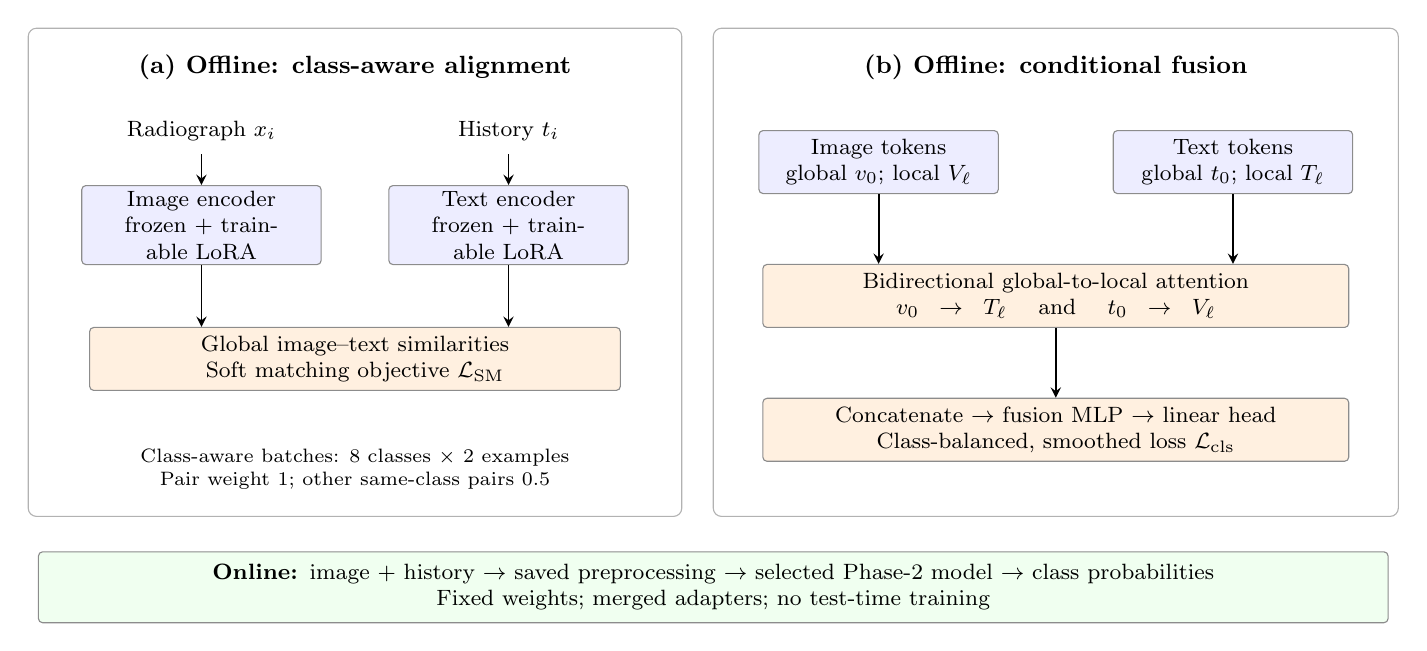
\begin{tikzpicture}[x=1mm,y=1mm,font=\footnotesize,
box/.style={draw=black!45,rounded corners=1.5pt,align=center,minimum height=8mm,inner sep=2pt},
flow/.style={->,>=stealth,line width=.65pt},
enc/.style={box,fill=blue!7,text width=29mm},
learn/.style={box,fill=orange!12},
note/.style={font=\scriptsize,align=center}]
\draw[rounded corners=3pt,draw=black!30] (0,0) rectangle (83,62);
\draw[rounded corners=3pt,draw=black!30] (87,0) rectangle (174,62);
\node[font=\small\bfseries] at (41.5,57) {(a) Offline: class-aware alignment};
\node[font=\small\bfseries] at (130.5,57) {(b) Offline: conditional fusion};
\node at (22,49) {Radiograph $x_i$};
\node at (61,49) {History $t_i$};
\node[enc] (vi) at (22,37) {Image encoder\\frozen + trainable LoRA};
\node[enc] (ti) at (61,37) {Text encoder\\frozen + trainable LoRA};
\draw[flow] (22,46) -- (vi);
\draw[flow] (61,46) -- (ti);
\node[learn,text width=66mm] (align) at (41.5,20) {Global image--text similarities\\Soft matching objective $\mathcal L_{\mathrm{SM}}$};
\draw[flow] (vi.south) -- (align.north -| vi.south);
\draw[flow] (ti.south) -- (align.north -| ti.south);
\node[note] at (41.5,6) {Class-aware batches: 8 classes $\times$ 2 examples\\Pair weight 1; other same-class pairs 0.5};
\node[enc] (vf) at (108,45) {Image tokens\\global $v_0$; local $V_\ell$};
\node[enc] (tf) at (153,45) {Text tokens\\global $t_0$; local $T_\ell$};
\node[learn,text width=73mm] (cross) at (130.5,28) {Bidirectional global-to-local attention\\$v_0\!\to\!T_\ell$ \quad and \quad $t_0\!\to\!V_\ell$};
\draw[flow] (vf.south) -- (cross.north -| vf.south);
\draw[flow] (tf.south) -- (cross.north -| tf.south);
\node[learn,text width=73mm] (head) at (130.5,11) {Concatenate $\to$ fusion MLP $\to$ linear head\\Class-balanced, smoothed loss $\mathcal L_{\mathrm{cls}}$};
\draw[flow] (cross) -- (head);
\node[box,fill=green!6,text width=170mm,minimum height=9mm] at (87,-9) {\textbf{Online:} image + history $\to$ saved preprocessing $\to$ selected Phase-2 model $\to$ class probabilities\\Fixed weights; merged adapters; no test-time training};
\end{tikzpicture}

\caption{Offline adaptation of XBone-Net. Phase 1 learns adapters from soft image--text matching targets; Phase 2 initializes from those adapters and learns bidirectional fusion and the classifier. The selected Phase-2 model supplies fixed-weight online inference.}
\label{fig:framework}
\end{figure*}

\subsection{Phase 1: Class-Aware Image--Text Alignment}
Each full batch contains two examples from each of eight sampled classes. This supplies same-class alternatives in addition to the original image--history pairs. For batch size $B$, define unnormalized matching weights
\begin{equation}
S_{ij}=\ind[i=j]+\rho\ind[i\ne j,\ y_i=y_j],\quad \rho=0.5.
\end{equation}
The original pair receives weight one; a different pair of the same class receives partial weight. Row and column normalization yield
\begin{equation}
Q^{I\to T}_{ij}=\frac{S_{ij}}{\sum_k S_{ik}},\qquad
Q^{T\to I}_{ji}=\frac{S_{ij}}{\sum_k S_{kj}}.
\end{equation}
Given normalized global embeddings $\bar v_i,\bar t_j$, the logits are $C_{ij}=e^s\bar v_i^\top\bar t_j$, with the pretrained logit scale $s$ fixed. Row-wise softmax of $C$ and $C^\top$ gives $P^{I\to T}$ and $P^{T\to I}$. We optimize
\begin{equation}
\mathcal L_{\mathrm{SM}}=-\frac{1}{2B}\sum_{i,j}
\left[Q^{I\to T}_{ij}\log P^{I\to T}_{ij}
+Q^{T\to I}_{ji}\log P^{T\to I}_{ji}\right].
\label{eq:align}
\end{equation}
This objective encourages class-consistent correspondence while preserving the observed pair as the strongest match. Class equality remains a coarse prior: it does not imply identical anatomy, severity, or clinical history.

\subsection{Phase 2: Bidirectional Fusion and Classification}
Native image and text tokens are layer-normalized and projected to 512 dimensions. Denote their additionally normalized global tokens by $v_0,t_0$ and remaining sequences by $V_\ell,T_\ell$. Each global token queries the other modality's local sequence through eight-head attention:
\begin{equation}
\begin{aligned}
h_I&=\operatorname{LN}\big(v_0+\operatorname{Drop}(\operatorname{MHA}(v_0,T_\ell,T_\ell;M_T))\big),\\
h_T&=\operatorname{LN}\big(t_0+\operatorname{Drop}(\operatorname{MHA}(t_0,V_\ell,V_\ell))\big),
\end{aligned}
\label{eq:fusion}
\end{equation}
where $M_T$ masks text padding. Thus, image context conditions the selection of text features and history conditions the selection of visual features. The summaries are concatenated, transformed by a $1024\to512\to512$ MLP with GELU and dropout, and classified:
\begin{equation}
z=\operatorname{LN}(\operatorname{MLP}([h_I;h_T])),\quad
p=\operatorname{softmax}(W_cz+b_c).
\end{equation}
The linear output head maps the learned fused representation to $K$ classes; linear separability is not assumed.

For training-class count $n_c$, the effective number is $E_c=(1-\beta^{n_c})/(1-\beta)$, with $\beta=0.999$. Inverse effective-number weighting and label smoothing give
\begin{equation}
\begin{aligned}
a_c&=E_c^{-1}, &w_c&=\min\left(\frac{Ka_c}{\sum_j a_j},5\right),\\
u_{ic}&=(1-\epsilon)\ind[y_i=c]+\epsilon/K, &\epsilon&=0.1,\\
\mathcal L_{\mathrm{cls}}&=-\frac{\sum_i\sum_c w_cu_{ic}\log p_{ic}}{\sum_i w_{y_i}}.&&
\end{aligned}
\label{eq:loss}
\end{equation}
Weights are computed from training data only and apply to all smoothed target terms. Phase~2 updates adapters, fusion, and the classifier. Weighting increases the influence of less frequent classes; smoothing regularizes the target distribution. Their individual effects on rare-class recall and probability calibration require separate evaluation.

\subsection{Input-Dependence Analysis}
After training, IG~\cite{Sundararajan2017IntegratedGradients} attributes the predicted-class logit $F_{\hat y}$ to each input component relative to reference $u^0$:
\begin{equation}
\operatorname{IG}_j(u;u^0)=(u_j-u_j^0)\int_0^1
\frac{\partial F_{\hat y}(u^0+\lambda(u-u^0))}{\partial u_j}\,d\lambda.
\end{equation}
We hold the other modality fixed and retain the original predicted class during intervention. Image deletion replaces ranked patches with the normalized zero reference; text deletion replaces content embeddings with padding embeddings while preserving special tokens and masks. Deletion AUC integrates predicted-class probability over the fraction removed. Whole-source replacement additionally measures $\Delta p_m=p_{\hat y}(x,t)-p_{\hat y}((x,t)_{\setminus m})$. These measures describe model dependence under specified interventions.

\section{Experiments}
\subsection{Experimental Setup}
Each reported classification result aggregates independent training runs with seeds 42, 123, and 456. Table~\ref{tab:setup} specifies the XBone-Net recipe. Checkpoints minimize validation loss in Phase~1 and maximize validation Macro-F1 in Phase~2. Images use BiomedCLIP's native RGB resize, center crop to $224\times224$, and normalization; text uses its tokenizer with maximum length 256. No additional lesion crops or image branches are used.

\begin{table}[t]
\caption{XBone-Net training configuration. Epoch counts are maxima; patience is in validation evaluations.}
\label{tab:setup}
\centering\footnotesize
\begin{tabularx}{\columnwidth}{@{}lY@{}}
\toprule
Setting & Value \\
\midrule
Hardware / precision & NVIDIA RTX 5060 Ti / BF16 \\
Optimizer / schedule & AdamW / cosine decay \\
Batch / accumulation & 16 / 1 \\
Weight decay & $10^{-4}$ \\
Phase 1 & 30 epochs; LR $5\times10^{-5}$; patience 3 \\
Phase 2 & 50 epochs; LR $10^{-4}$; patience 5 \\
LoRA & Rank 16; scaling 32; dropout 0.1 \\
Fusion & 512 dimensions; 8 heads; dropout 0.1 \\
Loss & $\rho=0.5$, $\beta=0.999$, $\epsilon=0.1$; weight cap 5 \\
\bottomrule
\end{tabularx}
\end{table}

\subsection{Datasets}
\textbf{CTCH} contains 3,249 radiograph--history pairs in 22 classes, including normal findings and fracture categories, from a single orthopedic hospital in Ho Chi Minh City. The patient-level split comprises 2,265 training, 315 validation, and 669 test cases with no shared patient keys. Text combines the reason for admission, disease history, and personal medical history, translated from Vietnamese into English. Explicit diagnostic-label and radiographic-finding fields are excluded. Prior diagnoses can nevertheless occur within history, and terminology may be affected by translation. The data are de-identified and used under a research confidentiality agreement; source clinical records are not publicly released.

\textbf{BTXRD}~\cite{Yao2025} contains 3,746 images in our ten-class formulation of normal findings and bone-tumor categories, with a 2,621/375/750 image-level split. Stable patient identifiers are unavailable for this partition. Text is generated from metadata conditioned on disease groups. Consequently, this experiment evaluates the recipe with label-correlated synthetic text; it does not independently establish the benefit of real clinical histories.

Table~\ref{tab:datasets} characterizes imbalance in the test cohorts. The largest classes contain 32.6\% of CTCH cases and 48.8\% of BTXRD images, whereas the smallest contain only six and nine cases. We therefore report Macro-F1 and balanced accuracy alongside accuracy. Macro-F1 averages class F1 scores; balanced accuracy averages class recalls. Classification results are reported as mean $\pm$ sample SD across three training seeds on the same split.

\begin{table}[t]
\caption{Dataset partitions and test-class support. Ratio is the largest divided by the smallest test-class count.}
\label{tab:datasets}
\centering\footnotesize
\begin{tabular}{@{}lcc@{}}
\toprule
Property & CTCH & BTXRD \\
\midrule
Classes & 22 & 10 \\
Train / validation / test & 2265 / 315 / 669 & 2621 / 375 / 750 \\
Split unit & Patient & Image \\
Text source & Clinical history & Synthetic metadata \\
Test count: min / median / max & 6 / 18.5 / 218 & 9 / 35.5 / 366 \\
Max/min ratio & $36.3\times$ & $40.7\times$ \\
\bottomrule
\end{tabular}
\end{table}

\subsection{Multimodal Image Classification}
Table~\ref{tab:classification} compares six locally trained baselines: ResNet-50 and DenseNet-121 use images only; CLIP, MedCLIP, PubMedCLIP~\cite{PubMedCLIP}, and BiomedCLIP use image--text pairs with full encoder tuning and global feature concatenation. Fully tuned BiomedCLIP uses learning rate $2\times10^{-5}$. These comparisons evaluate complete adaptation recipes rather than a controlled backbone substitution. The CTCH Image-only variant additionally removes history, Phase~1, and cross-modal fusion.

\begin{table*}[t]
\caption{Classification performance (\%, mean $\pm$ SD across three seeds). Best results are bold; second-best results are underlined. The proposed configurations are separated from the six baselines and their names are bold.}
\label{tab:classification}
\centering\footnotesize
\setlength{\tabcolsep}{6pt}
\begin{tabular*}{\textwidth}{@{\extracolsep{\fill}}lcccccc@{}}
\toprule
Method & \multicolumn{3}{c}{CTCH (22 classes; $n=669$)} & \multicolumn{3}{c}{BTXRD (10 classes; $n=750$)} \\
\cmidrule(lr){2-4}\cmidrule(l){5-7}
 & Accuracy & Balanced acc. & Macro-F1 & Accuracy & Balanced acc. & Macro-F1 \\
\midrule
ResNet-50 & $49.83\pm0.77$ & $41.80\pm0.46$ & $41.54\pm0.20$ & $60.67\pm1.33$ & $31.80\pm1.31$ & $32.85\pm0.96$ \\
DenseNet-121 & $48.18\pm0.38$ & $49.20\pm4.65$ & $43.60\pm2.42$ & $63.20\pm0.13$ & $36.94\pm1.50$ & $37.18\pm1.73$ \\
CLIP & $58.74\pm2.09$ & $\mathbf{62.17\pm3.59}$ & $\underline{56.33\pm0.90}$ & $80.36\pm2.73$ & $59.57\pm1.60$ & $57.87\pm2.52$ \\
MedCLIP & $56.00\pm3.96$ & $57.23\pm1.77$ & $51.61\pm2.24$ & $82.09\pm1.47$ & $\mathbf{61.27\pm2.38}$ & $\underline{60.57\pm1.53}$ \\
PubMedCLIP & $55.21\pm2.34$ & $55.89\pm6.14$ & $52.03\pm2.64$ & $78.84\pm2.85$ & $60.89\pm3.42$ & $57.23\pm5.77$ \\
BiomedCLIP & $\underline{59.69\pm2.53}$ & $\underline{60.23\pm2.34}$ & $55.40\pm0.80$ & $\mathbf{83.11\pm0.28}$ & $60.62\pm2.54$ & $59.94\pm1.24$ \\
\midrule
\textbf{XBone-Net Image-only (ours)} & $44.39\pm6.89$ & $48.43\pm1.36$ & $38.13\pm5.51$ & $64.23\pm1.54$ & $32.67\pm1.69$ & $40.21\pm2.57$ \\
\textbf{XBone-Net (ours)} & $\mathbf{61.83\pm2.03}$ & $59.35\pm1.34$ & $\mathbf{57.27\pm1.93}$ & $\underline{83.02\pm0.98}$ & $\underline{61.15\pm1.40}$ & $\mathbf{62.40\pm1.18}$ \\
\bottomrule
\end{tabular*}
\end{table*}


On CTCH, XBone-Net yields the highest observed accuracy and Macro-F1, with Macro-F1 gains of 1.87 percentage points over BiomedCLIP and 0.94 over CLIP. CLIP instead has higher balanced accuracy (62.17\% versus 59.35\%). On BTXRD, XBone-Net has the highest observed Macro-F1 (62.40\%), while BiomedCLIP and MedCLIP lead in accuracy and balanced accuracy, respectively. The gain is therefore metric dependent. The sizable gap between accuracy and Macro-F1 also indicates uneven class performance; higher aggregate Macro-F1 does not demonstrate improved recall for every rare diagnosis.

The CTCH resource profile in Table~\ref{tab:cost} quantifies the practical trade-off. XBone-Net updates 8.45M parameters, approximately 95.7\% fewer than full tuning, and lowers mean peak allocated training memory from 3816.8 to 1455.0 MiB. This reduces memory demand during local adaptation. However, training takes 2.50 times as long and measured inference latency rises from 13.77 to 16.17 ms. Parameter efficiency therefore concerns the optimized state and training memory, rather than faster execution.

\begin{table}[t]
\caption{CTCH resource trade-off against full BiomedCLIP tuning. Training time and peak allocated memory are mean $\pm$ SD across three seeds; inference is profiled at seed 42.}
\label{tab:cost}
\centering\footnotesize
\begin{tabular}{@{}lcc@{}}
\toprule
Measure & BiomedCLIP & \textbf{XBone-Net (ours)} \\
\midrule
Training model parameters (M) & 196.44 & 204.35 \\
Trainable parameters (M) & 196.44 & 8.45 \\
Trainable fraction (\%) & 100.00 & 4.13 \\
Training time (GPU-hours) & $0.3411\pm0.0800$ & $0.8542\pm0.0925$ \\
Peak allocated memory (MiB) & $3816.8\pm0.0$ & $1455.0\pm43.0$ \\
\midrule
Inference parameters (M) & 196.44 & 199.34 \\
GFLOPs & 81.03 & 82.32 \\
Latency (ms) & 13.77 & 16.17 \\
Throughput (samples/s) & 75.6 & 64.1 \\
\bottomrule
\end{tabular}
\end{table}

Training costs include both phases and their validation/checkpoint operations, excluding model loading and data-loader construction. Inference uses merged LoRA weights, BF16, and batch size one on the same GPU: 20 inputs, each with ten warm-up and ten timed forwards. Latency excludes data loading and host-to-device transfer; it is not end-to-end clinical workflow time.

\subsection{Ablation Study}
We compare internal CTCH variants on the same 669 test cases and three seeds. Phase~2 only omits alignment, while Concatenation replaces bidirectional cross-attention with global concatenation. Table~\ref{tab:ablation} isolates these architecture comparisons; the Image-only control is reported in Table~\ref{tab:classification}.

\begin{table}[t]
\caption{CTCH architecture ablations (\%, mean $\pm$ SD across three seeds). Best results are bold; second-best results are underlined. The Image-only control is reported in Table~\ref{tab:classification}.}
\label{tab:ablation}
\centering\footnotesize
\setlength{\tabcolsep}{3.5pt}
\begin{tabular}{@{}lccc@{}}
\toprule
Configuration & Accuracy & Balanced acc. & Macro-F1 \\
\midrule
\textbf{XBone-Net (ours)} & $\mathbf{61.83\pm2.03}$ & $\underline{59.35\pm1.34}$ & $\mathbf{57.27\pm1.93}$ \\
Phase 2 only & $\underline{60.04\pm0.85}$ & $55.52\pm3.41$ & $\underline{54.97\pm1.84}$ \\
Concatenation & $58.25\pm0.38$ & $\mathbf{59.83\pm2.68}$ & $54.77\pm1.62$ \\
\bottomrule
\end{tabular}
\end{table}


Removing Phase~1 lowers mean Macro-F1 by 2.30 percentage points; substituting concatenation lowers it by 2.50. Concatenation retains slightly higher balanced accuracy. These observations motivate alignment and conditional fusion, but the experiment does not establish their independent benefit across other splits or institutions. The 19.14-point Macro-F1 difference between full and Image-only configurations reflects the combined change in text access, alignment, and fusion. Isolated loss, sampler, and history-replacement experiments are needed to identify which mechanisms drive the difference.

\subsection{Image--Text Relationship Analysis}
We next examine how the trained model uses its two inputs. The analysis covers all 669 CTCH test cases at seed 42, including incorrect predictions, with 24 IG interpolation points. Image interventions operate on $16\times16$ patches; text interventions operate on content units. The other modality remains fixed. Each random deletion curve averages 16 orders per case, and each model retains its own original predicted class as the target.

Figure~\ref{fig:ig} shows lower targeted than random deletion AUC for images (0.2997 versus 0.3405) and text (0.2811 versus 0.3588). Thus, the attributed features in each modality are more influential under this intervention than randomly ordered features. Replacing the entire image decreases predicted-class probability by 0.3187 on average; replacing text decreases it by 0.2725. Together, these tests show aggregate dependence on both inputs. They do not establish semantic correctness of individual region--word correspondences or quantify interaction between modalities. The two deletion gaps also cannot rank modalities directly because their intervention units and references differ.

XBone-Net has image insertion AUC 0.4023, compared with 0.2517 for Image-only, but higher image deletion AUC (0.2997 versus 0.1541). Raw AUCs across models also depend on their starting confidence and selected target class. We therefore interpret these results as descriptive evidence about input use rather than a general advantage in explanation quality. For healthcare applications, this analysis supplies an auditable account of sensitivity to history and image content; lesion annotations, controlled history perturbations, and clinician review are needed to assess clinical plausibility.

\begin{figure*}[t]
\centering
\begin{tikzpicture}
\begin{groupplot}[
group style={group size=2 by 1,horizontal sep=13mm},
width=.46\textwidth,height=47mm,
xmin=0,xmax=1,ymin=0,ymax=.65,
xtick={0,.5,1},ytick={0,.2,.4,.6},
xlabel={Fraction removed},
axis lines=left,axis line style={black!60},
ymajorgrids,grid style={black!12},
tick label style={font=\footnotesize},
label style={font=\footnotesize},title style={font=\small\bfseries},
legend style={font=\scriptsize,draw=none,fill=none,at={(.98,.98)},anchor=north east},
]
\nextgroupplot[title={(a) Image patches},ylabel={Predicted-class probability}]
\addplot[color=red!70!black,line width=1.1pt] table[x=fraction,y=targeted]{ig_image.dat};
\addplot[color=blue!65!black,line width=1pt,dashed] table[x=fraction,y=random]{ig_image.dat};
\node[anchor=south west,font=\footnotesize,align=left] at (axis cs:.035,.025) {AUC gap: 0.0409};
\nextgroupplot[title={(b) Clinical-text units}]
\addplot[color=red!70!black,line width=1.1pt] table[x=fraction,y=targeted]{ig_text.dat};
\addlegendentry{IG-targeted deletion}
\addplot[color=blue!65!black,line width=1pt,dashed] table[x=fraction,y=random]{ig_text.dat};
\addlegendentry{Random deletion}
\node[anchor=south west,font=\footnotesize] at (axis cs:.035,.025) {AUC gap: 0.0777};
\end{groupplot}
\end{tikzpicture}

\caption{IG-guided deletion on all 669 CTCH test cases at seed 42. Curves average the probability of each case's original predicted class; the comparison averages 16 random orders per case. AUC gaps are random minus targeted deletion AUC. Each modality is perturbed while the other remains fixed.}
\label{fig:ig}
\end{figure*}

\section{Limitations and Conclusion}
XBone-Net combines class-aware alignment, low-rank adaptation, and bidirectional fusion for radiograph--history classification. It achieves competitive Macro-F1 while substantially reducing trainable parameters and allocated training memory, with longer training and higher CTCH inference latency. The application-level contribution is a measured adaptation trade-off accompanied by architecture and input-dependence analyses.

The evaluation uses fixed splits and three training seeds, a single-center clinical cohort, and synthetic BTXRD text. It therefore does not measure variation across hospitals, alternative patient splits, or real histories on BTXRD. The input analysis uses one seed; rare-class sensitivity, translation quality, and residual diagnostic information in histories need further study. Direct prompt-learning comparisons and independently controlled component ablations are also absent. These retrospective results do not establish clinical deployment readiness.

Future work will evaluate a fixed model on independent patient cohorts, isolate alignment and fusion effects, and test missing, mismatched, or contradictory histories. Multi-scale imaging and per-class error analysis may clarify performance on small lesions and rare categories. Repeating IG with different references and seeds, followed by lesion-region and clinician assessment, can test explanation stability and plausibility. Simplified fusion, distillation, and quantization should be evaluated jointly against accuracy, memory, and latency before prospective studies with clinician supervision.

\section*{Acknowledgment}
OpenAI Codex assisted language revision of the Abstract and Sections I--V, LaTeX preparation, and plotting of existing results. Experimental predictions were not generated by the writing tool; the authors are responsible for final verification.

\bibliographystyle{IEEEtran}
\IEEEtriggeratref{10}
\bibliography{references}
\end{document}
